
%%==================================================
%% demo.tex for BIT Thesis
%% modified by yang yating
%% version: 1.2
%% last update: Jan. 4th, 2018
%%==================================================

% 默认单面打印 oneside 、硕士论文模板 master

\documentclass[oneside, master]{BIT-thesis-grd}

% 模板选项: 硕士论文 master; 博士论文 doctor

%==============更改数学字体设置,Latin Modern Math 默认的的确有点细,看个人需要,下面提供一种方法,需要的可以取消注释=========%

% \usepackage[bold-style=ISO]{unicode-math} %采用unicode-math,可以直接输入Unicode公式,当然传统的输入就行
% \setmathfont{XITS Math}  %目前unicode-math 支持几种数学字体,具体用法可以查看帮助文档,这里采用类似times字体科学数学字体,可以取消注释对比


\begin{document}

%%%%%%%%%%%%%%%%%%%%%%%%%%%%%%
%% 封面
%%%%%%%%%%%%%%%%%%%%%%%%%%%%%%

% 中文封面内容(关注内容而不是表现形式)
\classification{TQ028.1}
\UDC{540}

\title{形状记忆聚氨酯的合成及其在织物中的应用}
\vtitle{形状记忆聚氨酯的合成及其在织物中的应用}
\author{***}
\institute{**学院}
\advisor{**教授}
\chairman{**教授}
\degree{工学硕士(博士)}
\major{*****}
\school{北京理工大学}
\defenddate{****年*月}
%\studentnumber{**********}


% 英文封面内容(关注内容而不是表现形式)
\englishtitle{Synthesis and Application on textile of the Shape\\Memory Polyurethane}
\englishauthor{***}
\englishadvisor{Prof. **}
\englishchairman{Prof. **}
\englishschool{Beijing Institute of Technology}
\englishinstitute{****}
\englishdegree{****}
\englishmajor{****}
\englishdate{*,****}

% 封面绘制
\maketitle

% 中文信息
\makeInfo

% 英文信息
\makeEnglishInfo

%打印竖排论文题目
\makeVerticalTitle

% 论文原创性声明和使用授权
\makeDeclareOriginal

%%%%%%%%%%%%%%%%%%%%%%%%%%%%%%
%% 前置部分
%%%%%%%%%%%%%%%%%%%%%%%%%%%%%%
\frontmatter

% 摘要
%%==================================================
%% abstract.tex for BIT Master Thesis
%% modified by yang yating
%% version: 0.1
%% last update: Dec 25th, 2016
%%==================================================

\begin{abstract}

本文主要的研究内容为固定翼无人机紧密编队控制器设计。该控制器以固定翼无人机编队的领从方法(leader-follower method)为基础,并考虑
内环的姿态驾驶仪的控制输入量,完成从编队误差量到姿态控制输入量的计算。
初步设计完成之后,再从无人机的动力学模型出发,使用MATLAB/Simulink等数学仿真工具研究控制器设计的稳定性以及动态特性。
其次选取合适的无人机飞行平台,飞行控制硬件并编写控制程序,完成飞行实验验证。完成编队控制器的参数参数整定之后,将实验的结果与仿真结果相对比,
最后,使用改进后的编队控制器完成双机编队任务,研究编队过程中的空气动力效果问题,
即研究此尺寸无人机编队群对提高整体飞行效率的作用。
%TODO:这里的研究目的要针对研究情况改写。
%({\color{blue}{摘要是一篇具有独立性和完整性的短文,应概括而扼要地反映出本论文的主要内容。包括研究目的、研究方法、研究结果和结论等,特别要突出研究结果和结论。中文摘要力求语言精炼准确,硕士学位论文摘要建议500$\sim$800字,博士学位论文建议1000$\sim$1200字。摘要中不可出现参考文献、图、表、化学结构式、非公知公用的符号和术语。英文摘要与中文摘要的内容应一致。}})

\keywords{固定翼无人机、领从方法、编队控制器设计、紧密编队控制、编队空气动力学、飞行实验}
%({\color{blue}{一般选3~8个单词或专业术语,且中英文关键词必须对应。})}}
\end{abstract}

\begin{englishabstract}

The main content of this thesis is to design the close formation controller adapted to the inner-loop attitude controller of
the fixed-wing UAV, which is based on the leader-follower method of the UAV formation control. The close formation controller 
plays role of translating the formation errors to the input of the inner loop
attitude controller. After the preliminary design of the formation controller, the MATLAB/Simulink is used to test and verify the 
dynamic quality and stability. After that, the controller is rewrote to the algorithm running on the upper controller. The hardware
of the controller and the UAV platform is well chosen to accomplish the formation experiment. During this period, the parameters are 
tuned in order to accomplish the optimal control effect.
Finally, the double fixed-wing UAV formation is conducted to verify the effect of the flight efficiency produced by the close formation.
   
\englishkeywords{fixed-wing UAV, leader-follower method, formation controller design, close formation control, formation aerodymatic, flight experiment}

\end{englishabstract}

%% 符号对照表,可选,如不用可注释掉
\begin{denotation}
	
\item[BIT] 北京理工大学的英文缩写
\item[\LaTeX] 一个很棒的排版系统
\item[\LaTeXe] 一个很棒的排版系统的最新稳定版
\item[\XeTeX] \LaTeX{}的好兄弟,事实上他有很多个兄弟,但是这个兄弟对各种语言的支持能力都很强
\item[ctex] 成套的中文\LaTeX{}解决方案,由一帮天才们开发
\item[\ce{H2SO4}] 硫酸
\item[$ e^{\pi{}i}+1=0$] 一个集自然界五大常数一体的炫酷方程
\item[\ce{2H2 + O2 -> 2H2O}] 一个昂贵的生成生命之源的方程式

\end{denotation}

% 加入目录
\tableofcontents


%加入图、表索引(同时取消图表索引中章之间的垂直间隔)
\let\origaddvspace\addvspace
\renewcommand{\addvspace}[1]{}
\listoffigures
\listoftables
\renewcommand{\addvspace}[1]{\origaddvspace{#1}}



%%%%%%%%%%%%%%%%%%%%%%%%%%%%%%
%% 正主体部分
%%%%%%%%%%%%%%%%%%%%%%%%%%%%%%
\mainmatter

%% 各章正文内容
%%==================================================
%% chapter01.tex for BIT Master Thesis
%% modified by yang yating
%% version: 0.1
%% last update: Dec 25th, 2016
%%==================================================
\chapter{绪论}
\label{chap:intro}
\section{本论文研究的目的和意义}

在未来战争中,仅靠单架无人机自主作战无法适应复杂多样的战场环境,而具备协同作战的无人机编队能更好地完成任务,与单架无人机相比具有作战效率高、
视野广阔等优势,可实现对目标的全方位立体监视,对地精确攻击。另外,无人机紧密编队可以实现长航任务中无人机的空中加油,对接等任务,如图\ref{fig:c01-meaning-1}。编队飞行作为
无人机研究领域的热点与难点问题,涉及多项关键技术,例如:队形设计、自主编队、队形保持变换、协调通信等。无人机自主编队控制是实现集群作战的关键技
术。

固定翼无人机以紧密编队的形式飞行,如迁徙的鸟儿一样,可以减少整体的飞行阻力并且减少燃料消耗。整体编队产生的效果将会与精心设计的、具有良好的气动
外形的飞行器相媲美。但是,按照相关文献显示,如果固定翼编队的控制精度无法达到要求精度的10\%,那么最优的减租效果可能会被削减30\%。
\begin{figure}
  \centering
  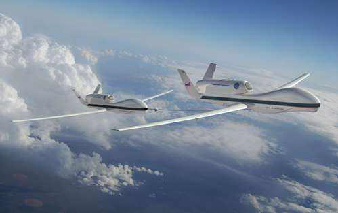
\includegraphics[width=0.75\textwidth]{figures/c01-meaning-1}
  \caption{无人机编队加受油}\label{fig:c01-meaning-1}
 \end{figure}

%\upcite{Takahashi1996Structure,Xia2002Analysis,Jiang1989,Mao2000Motion,Feng1998}%这个是文献引用上标
\section{国内外研究现状及发展趋势}
%\label{sec:***} 可标注label
现如今的无人机自动驾驶仪的结构多为导航模块、位置控制控制模块(外环)以及姿态控制模块(内环);导航模块产生期望位置,位置控制模块由期望位置产生
期望姿态角,姿态控制模块由期望姿态角产生最终的伺服系统的控制量。现如今的低成本无人机所使用的传感器硬件精度比较低,均为消费级别,如果不考虑传感
器的精度问题而设计控制方案,很可能导致整体编队的控制精度下降。现如今已经存在的大部分编队控制算法,未考虑无人机的动力学模型,即只考虑飞机的质点
运动学以及质点动力学条件下提出的导航方法,最终产生的飞行器的控制量为无人机航迹坐标系下的加速度期望值。按照飞机的控制方式,需要将航迹坐标系下的
期望控制量转到机体系之下,但是飞机自动驾驶仪并不能接受加速度控制量,尤其是飞机机体x轴方向,无人机推力、阻力以及重力沿机体方向的推力并非是代数关
系,不能直接由期望加速度得到期望推力;另外由于低成本无人机的惯性原件的精度问题导致无人机不能使用测量的加速度信息作为反馈,两种原因导致以加速度
为最终控制量对于低成本无人机编队的方法控制精度不足。目前的编队控制算法正在向考虑无人机动力学模型方向发展。

%\chapter{无人机编队的动力学模型的建立}
\label{chap:formation_dynamic_equ}
本章基于无人机编队的领从方法(leader-follower method)建立无人机编队的相对运动方程。为了与无人机的解耦控制方法相匹配,本文的
模型建立将无人机运动分为水平平面运动以及竖直平面运动内分别建立数学模型。由于无人机尺寸小,强度大,飞行包线较小,现做如下假设:
\begin{itemize}
    \item 无人机为具有6自由度的三维空间运动刚体。
    \item 忽略地球自转,将地球作为惯性系。
    \item 忽略地球曲率,即所谓的“平板地球假设”。%TODO:考虑是否要加入大气的假设,以及引用文献
    \item 由于内环控制率以无人机协调(倾斜)转弯(STT)为基础(详见第\ref{chap:hardware}章),飞机满足无侧滑条件,侧滑角为0;即空速方向与机体系$O_bx_b$在同一铅垂平面内。
\end{itemize}
本章中涉及的坐标系有:
\begin{enumerate}
    \item 地面坐标系$O_gx_gy_gz_g$:$O_g$选为无人机解锁时的位置,$O_gx_g$轴指向北,$O_gy_g$轴指向东,$O_gz_g$轴符合右手定则,指向下。
    \item 导航坐标系$NED(north-east-down)$:原点选做飞机质心,$N$轴指向北,$E$轴指向东,$D$轴符合右手定则,指向下。
    \item 航迹坐标系$O_kx_ky_kz_k$:$O_k$选为无人机质心,$O_kx_k$轴始终与无人机地速方向一致,$O_kz_k$轴位于包含$O_kx_k$轴的铅垂平面内,
    $o_ky_k$符合右手定则,指向右。
    \item 机体坐标系$O_bx_by_bz_b$:$O_b$选为无人机质心,$O_bx_b$位于无人机的对称平面内,平行于机身轴线或者机翼的平均气动弦线,指向前;$O_bz_b$亦在对称平面之内,
    垂直于$O_bx_b$轴,指向下;$O_by_b$垂直于对称平面,指向右。机体坐标系始终与无人机固连。
    \item 气流坐标系$O_ax_ay_az_a$:气流坐标系又被称作风坐标系或者速度坐标系;$O_a$取作无人机质心,$O_ax_a$始终指向无人机的空速方向;$O_az_a$位于无人机对称面之内,
    垂直于$O_ax_a$轴,指向下;$O_ay_a$轴垂直于$O_ax_az_a$平面,指向右。只有在大气风速$V_{wind}=0$时,航迹系的$O_kx_k$才与气流坐标系的$O_ax_a$重合。
\end{enumerate}

本章中领机与从机的各运动学量以及几何关系分别用上标$l,f$标记,从机期望值以$“des”$上标标记;
运动学量以及几何关系所属坐标系关系则用各个坐标系的字母作为下标标记。
领机、从机在水平以及竖直平面内的几何关系分别在图\ref{fig:c02-2d_level_motion}和图\ref{fig:c02-2d_vert_motion}给出;
\begin{figure}[H]
    \centering
    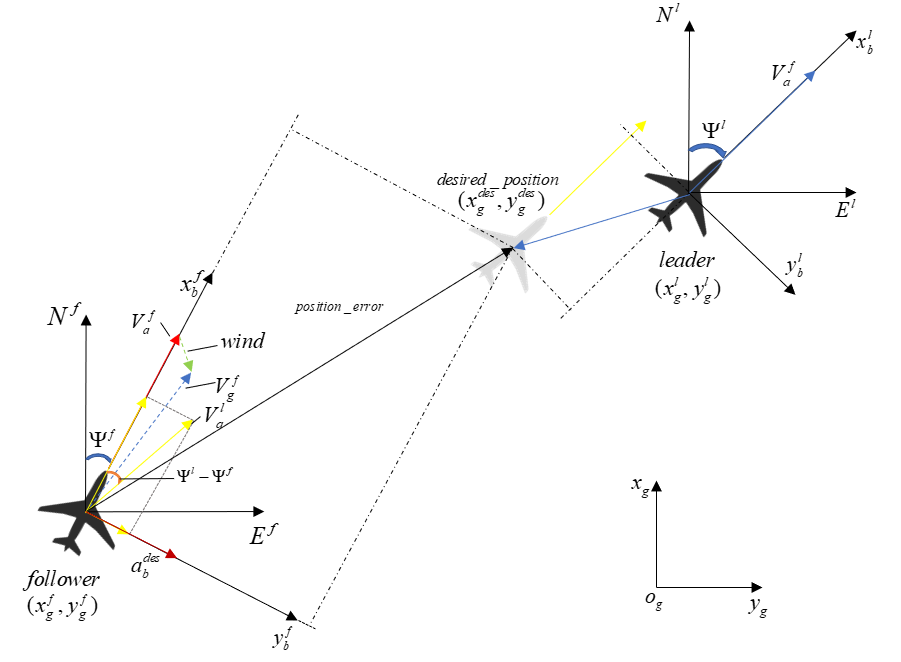
\includegraphics[width=0.75\textwidth]{figures/c2/2d_level_motion.png}
    \caption{水平平面双机编队几何关系}\label{fig:c02-2d_level_motion}
\end{figure}
\begin{figure}[H]
    \centering
    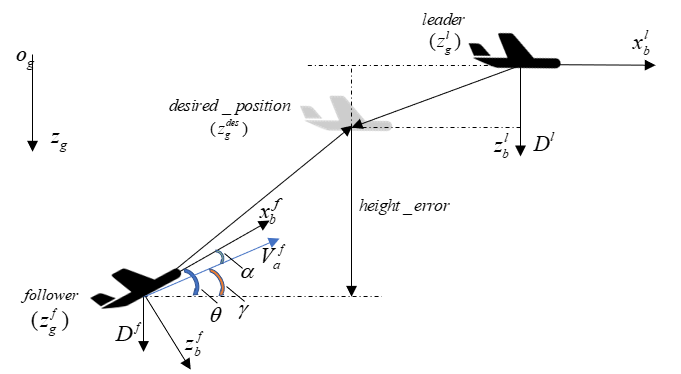
\includegraphics[width=0.75\textwidth]{figures/c2/2d_vert_motion.png}
    \caption{竖直平面双机编队几何关系}\label{fig:c02-2d_vert_motion}
\end{figure}
在图\ref{fig:c02-2d_level_motion}中:
$(x_{g}^l,y_{g}^l),(x_{g}^f,y_{g}^f),(x_{g}^{des},y_{g}^{des})$分别为领机、从机以及从机期望编队位置在地面坐标系$O_gx_gy_g$平面之中的分量;
$\Psi^l,\Psi^f$分别为领机与从机的偏航角(yaw angle);
$\chi^l,\chi^f$分别为领机与从机的航迹偏角(航迹方位角);
$V_a,V_{wind},V_g$分别为领机和从机的空速、风速以及地速向量;
$a_{b}^{des}$是从机产生的、在体轴系下的期望的法向加速度。

在图\ref{fig:c02-2d_vert_motion}中:
$z_{g}^l,,z_{g}^f,z_{g}^{des}$分别为领机、从机以及从机期望编队位置在地面坐标系$O_gz_g$轴上的分量;
$\theta^l,\theta^f$分别为领机与从机的俯仰角(pitch angle);
$\gamma^l,\gamma^f$分别为领机与从机的航迹倾角(航迹倾斜角);
$V_a,V_{wind},V_g$分别为领机和从机的空速、风速以及地速向量;

在图\ref{fig:c02-2d_level_motion}和图\ref{fig:c02-2d_vert_motion}中,由飞机飞行动力学可知,从机与领机三维运动学方程均为:
\begin{equation}
    \left\{
    \begin{array}{l}
        \frac{dx_g}{dt}=V_g\cos\gamma\cos\chi\\
        \frac{dy_g}{dt}=V_g\cos\gamma\sin\chi\\
        \frac{dz_g}{dt}=-V_g\sin\gamma
    \end{array}
    \right .
    \label{fol_motion_eauation}
\end{equation}
现考虑无风情况下,则由图\ref{fig:c02-2d_level_motion}可知,无人机航迹偏角等于航向角,即$\Psi=\chi$;无人机在平衡状态下,迎角很小(本无人机约在2.3°左右),由图\ref{fig:c02-2d_vert_motion}可得$\theta\approx\gamma$。
于是方程组\ref{fol_motion_eauation}可改写为:
\begin{equation}
    \left\{
    \begin{array}{l}
        \frac{dx_g}{dt}=V_g\cos\theta\cos\Psi\\
        \frac{dy_g}{dt}=V_g\cos\theta\sin\Psi\\
        \frac{dz_g}{dt}=-V_g\sin\theta
    \end{array}
    \right .
    \label{fol_motion_eauation1}
\end{equation}
方程组\ref{fol_motion_eauation1}的第1、2两式表示无人机在水平平面内的运动轨迹;第3式表示无人机在竖直平面内的运动轨迹。方程组中,控制的直接输入量为从机的$V_{g}^f,\theta^f,\Psi^f$,再确定飞机的初始运动量之后,可唯一确定领机与从机的
运动规律。

值得注意的是:上述控制量并不能直接由编队控制器产生,但经过理想内环控制器以及无人机动力学模型之后,将产生相应的上述的直接控制量,完整流程将在第\ref{chap:controller_design}章中介绍。
%\chapter{编队控制器设计}
\label{chap:controller_design}
第\ref{chap:formation_dynamic_equ}章中介绍了无人机双机编队的动力学模型,并将无人机运动分为铅垂平面以及水平平面;方程组\ref{fol_motion_eauation1}水平平面的直接输入量为$\Psi$的期望值,铅垂平面的
直接输入量为$\theta$和$V$的期望值。整体的控制逻辑框图如下图所示:
%TODO:此处加入整体的控制逻辑框图。
编队控制器的输入为定义的误差量,输出为无人机自动驾驶仪的内环输入值,即期望推力$T^{des}$,期望姿态$\Phi^{des},\theta^{des}$,偏航期望值$\Psi^{des}$将由内环姿态
自动驾驶仪按照协调转弯条件计算得到。本章的剩余部分将分别设计铅垂平面以及水平平面的控制器。
%TODO:此处的分配方式有些问题,考虑机体x和y
\section{水平平面编队控制器设计}
导航的本质是控制地速的方向,实现手段是产生垂直于速度方向的法向加速度;在无人机之中,多采用协调转弯(BTT)方式产生法向加速度。在导弹的制导规律之中,制导的最终目标是与期望的
点相交,而编队控制器的最终目标为:
\begin{enumerate}
    \item 从机速度方向与领机的速度方向一致。
    \item 从机的速度大小与领机的速度大小一致。
    \item 从机的位置与从机的期望位置一致。
\end{enumerate}
此处产生三种误差类型,这三类误差均投影在从机机体坐标系$O_bx_by_bz_b$之中,便于之后产生控制量:
\begin{enumerate}
    \item 领机与从机2维速度方向误差$\eta^{err}$。%TODO:记得改一下图,与之对应
    \item 领机与从机3维速度大小误差$(V_{X_b}^{err},V_{Y_b}^{err})$。
    \item 领机与从机3维位置误差$(P_{X_b}^{err},P_{Y_b}^{err},P_{Z_b}^{err})$
\end{enumerate}
因而此处水平平面的编队控制器的控制的任务是消除速度方向上的角度误差以及水平平面内的位置误差,即水平平面编队控制器应产生期望速度$V^{des}$以及期望法向加速度$a_{f}^{des}$。
\section{铅垂平面编队控制器设计}


%%==================================================
%% conclusion.tex for BIT Master Thesis
%% modified by yang yating
%% version: 0.1
%% last update: Dec 25th, 2016
%%==================================================


\begin{conclusion}

本文采用……。{\color{blue}(结论作为学位论文正文的最后部分单独排写,但不加章号。结论是对整个论文主要结果的总结。在结论中应明确指出本研究的创新点,对其应用前景和社会、经济价值等加以预测和评价,并指出今后进一步在本研究方向进行研究工作的展望与设想。结论部分的撰写应简明扼要,突出创新性。)}

\end{conclusion}

%% 参考文献,五号字,使用 BibTeX,包含参考文献文件.bib

%\bibliography{reference/chap1,reference/chap2} %多个章节的参考文献
\bibliography{reference/chap1}


%%%%%%%%%%%%%%%%%%%%%%%%%%%%%%
%% 后置部分
%%%%%%%%%%%%%%%%%%%%%%%%%%%%%%

%% 附录(章节编号重新计算,使用字母进行编号)
\appendix
\renewcommand\theequation{\Alph{chapter}--\arabic{equation}}  % 附录中编号形式是"A-1"的样子
\renewcommand\thefigure{\Alph{chapter}--\arabic{figure}}
\renewcommand\thetable{\Alph{chapter}--\arabic{table}}

%%==================================================
%% app1.tex for BIT Master Thesis
%% modified by yang yating
%% version: 0.1
%% last update: Dec 25th, 2016
%%==================================================


\chapter{***}

附录相关内容…
 

\chapter{Maxwell Equations}


因为在柱坐标系下,$\overline{\overline\mu}$是对角的,所以Maxwell方程组中电场$\bf
E$的旋度

所以$\bf H$的各个分量可以写为:
\begin{subequations}
  \begin{eqnarray}
    H_r=\frac{1}{\mathbf{i}\omega\mu_r}\frac{1}{r}\frac{\partial
      E_z}{\partial\theta } \\
    H_\theta=-\frac{1}{\mathbf{i}\omega\mu_\theta}\frac{\partial E_z}{\partial r}
  \end{eqnarray}
\end{subequations}
同样地,在柱坐标系下,$\overline{\overline\epsilon}$是对角的,所以Maxwell方程组中磁场$\bf
H$的旋度
\begin{subequations}
  \begin{eqnarray}
    &&\nabla\times{\bf H}=-\mathbf{i}\omega{\bf D}\\
    &&\left[\frac{1}{r}\frac{\partial}{\partial
        r}(rH_\theta)-\frac{1}{r}\frac{\partial
        H_r}{\partial\theta}\right]{\hat{\bf
        z}}=-\mathbf{i}\omega{\overline{\overline\epsilon}}{\bf
      E}=-\mathbf{i}\omega\epsilon_zE_z{\hat{\bf z}} \\
    &&\frac{1}{r}\frac{\partial}{\partial
      r}(rH_\theta)-\frac{1}{r}\frac{\partial
      H_r}{\partial\theta}=-\mathbf{i}\omega\epsilon_zE_z
  \end{eqnarray}
\end{subequations}
由此我们可以得到关于$E_z$的波函数方程:
\begin{eqnarray}
  \frac{1}{\mu_\theta\epsilon_z}\frac{1}{r}\frac{\partial}{\partial r}
  \left(r\frac{\partial E_z}{\partial r}\right)+
  \frac{1}{\mu_r\epsilon_z}\frac{1}{r^2}\frac{\partial^2E_z}{\partial\theta^2}
  +\omega^2 E_z=0
\end{eqnarray}
 

%(其后部分无编号)
\backmatter

% 发表文章目录
%%==================================================
%% pub.tex for BIT Master Thesis
%% modified by yang yating
%% version: 0.1
%% last update: Dec 25th, 2016
%%==================================================

\begin{publications}{99}

    \item\textsc{高凌}. {交联型与线形水性聚氨酯的形状记忆性能比较}[J].
      化工进展, 2006, 532-535.(核心期刊)
    
\end{publications}

% 致谢
%%==================================================
%% thanks.tex for BIT Master Thesis
%% modified by yang yating
%% version: 0.1
%% last update: Dec 25th, 2016
%%==================================================

\begin{thanks}

本论文的工作是在导师……。

\end{thanks}

% 作者简介(博士论文需要)
%%==================================================
%% resume.tex for BIT Master Thesis
%% modified by yang yating
%% version: 0.1
%% last update: Dec 25th, 2016
%%==================================================

\begin{resume}

本人…。

\end{resume}



\end{document}
